\begin{figure}[!htbp]
\centering
\vspace{1\baselineskip}
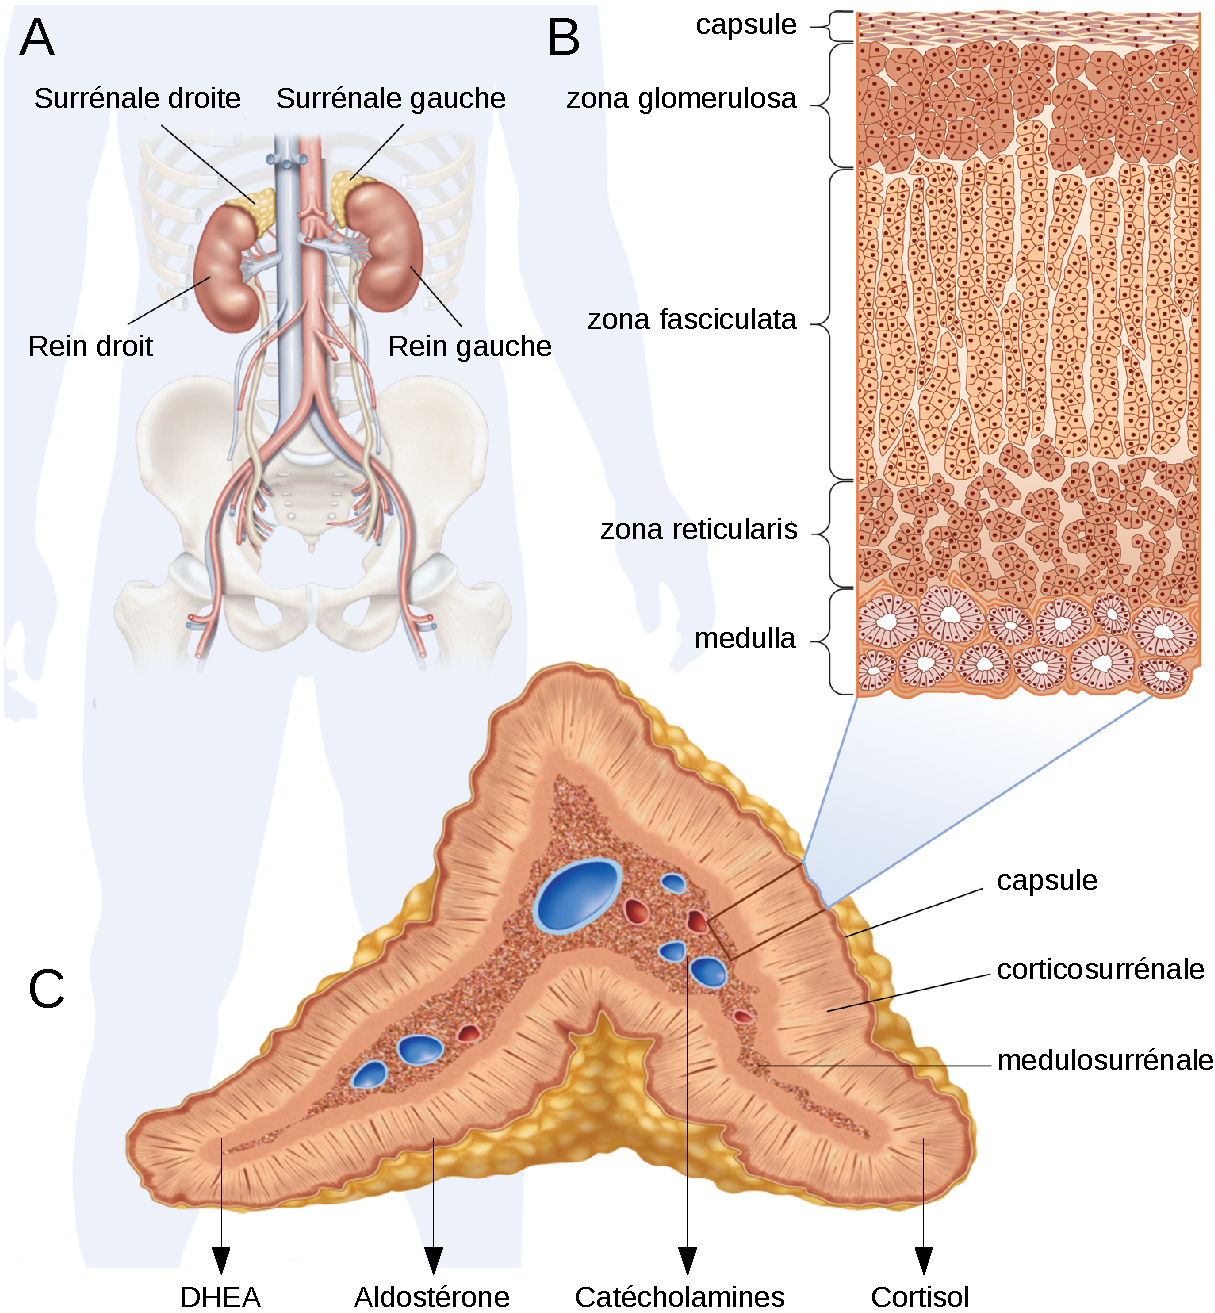
\includegraphics[width=\textwidth]
{Figures/adrenal-gland/adrenal-gland.pdf}
\caption[Les glandes surrénales]
{
Schéma des glandes surrénales.
Les glandes surrénales sont deux glandes situées au dessus des reins.
Elles sont entourées de la capsule, qui maintient leur structure.
La \textit{medulla} est la partie centrale des surrénales et compose les médullosurrénales.
C'est dans cette structure que les cellules chromaffines (en bleu) produisent les catécholamines sous forme d'adrénaline et de noradrénaline.
Le cortex compose les glandes corticosurrénales.
Il est subdivisé en trois couches, la \textit{zona glomerulosa} où sont produits les \glspl{mc}, la \textit{zona fasciculata} produisant essentiellement les \glspl{gc} et la \textit{zona reticularis} produisant essentiellement des hormones androgènes et une partie des \glspl{gc}.
Peu de stockage a lieu, et les hormones synthétisées sont immédiatement libérées dans la circulation sanguine.
Figure adaptée de Encyclopaedia Britannica.
}
\label{fig:adrenal-gland}
\end{figure}